\let\negmedspace\undefined
\let\negthickspace\undefined
\documentclass[journal,12pt,onecolumn]{IEEEtran}
\usepackage{cite}
\usepackage{amsmath,amssymb,amsfonts,amsthm}
\usepackage{algorithmic}
\usepackage{graphicx}
\graphicspath{{./figs/}}
\usepackage{textcomp}
\usepackage{xcolor}
\usepackage{txfonts}
\usepackage{listings}
\usepackage{enumitem}
\usepackage{mathtools}
\usepackage{gensymb}
\usepackage{comment}
\usepackage{caption}
\usepackage[breaklinks=true]{hyperref}
\usepackage{tkz-euclide} 
\usepackage{listings}
\usepackage{gvv}                                        
%\def\inputGnumericTable{}                                 
\usepackage[latin1]{inputenc}     
\usepackage{xparse}
\usepackage{color}                                            
\usepackage{array}
\usepackage{longtable}                                       
\usepackage{calc}                                             
\usepackage{multirow}
\usepackage{multicol}
\usepackage{hhline}                                           
\usepackage{ifthen}                                           
\usepackage{lscape}
\usepackage{tabularx}
\usepackage{array}
\usepackage{float}
\newtheorem{theorem}{Theorem}[section]
\newtheorem{problem}{Problem}
\newtheorem{proposition}{Proposition}[section]
\newtheorem{lemma}{Lemma}[section]
\newtheorem{corollary}[theorem]{Corollary}
\newtheorem{example}{Example}[section]
\newtheorem{definition}[problem]{Definition}
\newcommand{\BEQA}{\begin{eqnarray}}
\newcommand{\EEQA}{\end{eqnarray}}
\newcommand{\define}{\stackrel{\triangle}{=}}
\theoremstyle{remark}
\newtheorem{rem}{Remark}

\begin{document}

\title{5.2.59}
\author{ee25btech11057 - Tammineedi Rushil Shanmukha Srinivas}
\maketitle
\renewcommand{\thefigure}{\theenumi}
\renewcommand{\thetable}{\theenumi}


\textbf{Question :} Solve the system of equations

\begin{align}
2x +3y + 3z &= 5\\
x -2y +z &= -4\\
3x -y -2z &= 3
\end{align}


\textbf{Solution :}


The system of equations in matrix form is :

\begin{align}
  \myvec{2 & 3 & 3\\1 & -2 & 1\\3 & -1 & -2}\myvec{x\\y\\z} &= \myvec{5\\-4\\3}
\end{align}

Forming the augmented matrix,

\begin{align}
  \myaugvec{3}{2 & 3 & 3 & 5\\ 1 & -2 & 1 & -4\\3 & -1 & -2 & 3}
\end{align}

Using Gaussian elimination,

\begin{align}
  \myaugvec{3}{2 & 3 & 3 & 5\\ 1 & -2 & 1 & -4\\3 & -1 & -2 & 3}
  \xleftrightarrow[\;R_2 \to 2R_2 -R_1\;]{\;R_3 \to 2R_3 - 3R_1}
  \myaugvec{3}{2 & 3 & 3 & 5\\0 & -7 & -1 & -13\\0 & -11 & -13 & -9}
  \xleftrightarrow{R_3 \to R_3 -\tfrac{11}{7}R_2}
  \myaugvec{3}{2 & 3 & 3 & 5\\0 & -7 & -1 & -13\\0 & 0 & \tfrac{-80}{7} & \tfrac{80}{7}}
\end{align}

Using back substitution we get :

\begin{align}
  \tfrac{-80}{7} z &= \tfrac{80}{7}\\ 
  z &= -1\\
  -7y - z &= -13\\
  -7y +1 &= -13\\
  7y &= 14\\
  y &= 2\\
  2x + 3y + 3z &= 5\\
  2x + 3 &= 5\\
  x &= 1
\end{align}

\pagebreak

Therefore the solution for the system of equations is : 

\begin{align}
  \myvec{1\\2\\-1}
\end{align}


\begin{figure}[h!]
  \centering
  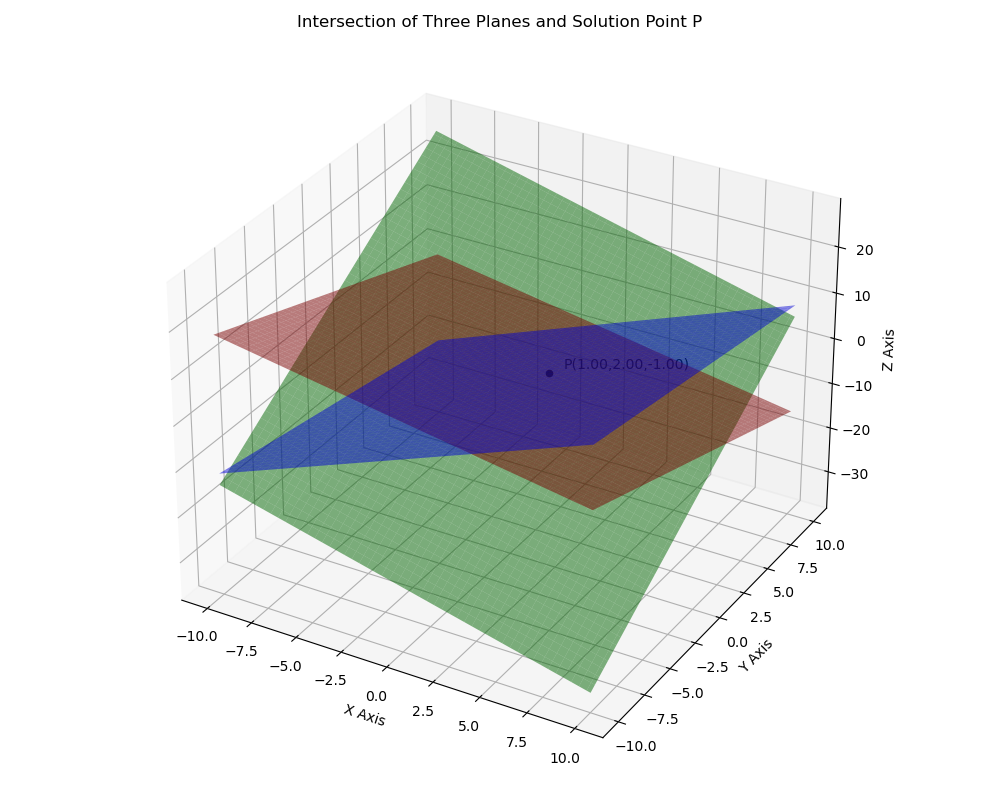
\includegraphics[width=0.9\columnwidth]{figs/solution.png} 
   \caption*{Fig : Planes}
  \label{Fig1}
\end{figure}


\end{document}
